% 
% Annual Cognitive Science Conference
% Sample LaTeX Paper -- Proceedings Format
% 

% Original : Ashwin Ram (ashwin@cc.gatech.edu)       04/01/1994
% Modified : Johanna Moore (jmoore@cs.pitt.edu)      03/17/1995
% Modified : David Noelle (noelle@ucsd.edu)          03/15/1996
% Modified : Pat Langley (langley@cs.stanford.edu)   01/26/1997
% Latex2e corrections by Ramin Charles Nakisa        01/28/1997 
% Modified : Tina Eliassi-Rad (eliassi@cs.wisc.edu)  01/31/1998
% Modified : Trisha Yannuzzi (trisha@ircs.upenn.edu) 12/28/1999 (in process)
% Modified : Mary Ellen Foster (M.E.Foster@ed.ac.uk) 12/11/2000
% Modified : Ken Forbus                              01/23/2004
% Modified : Eli M. Silk (esilk@pitt.edu)            05/24/2005
% Modified: Niels Taatgen (taatgen@cmu.edu) 10/24/2006

%% Change ``a4paper'' in the following line to ``letterpaper'' if you are
%% producing a letter-format document.

\documentclass[10pt,letterpaper]{article}
\usepackage{graphicx}
\usepackage{cogsci}
\usepackage{pslatex}
\usepackage{apacite}
\usepackage{amssymb,amsfonts,amsmath}
\usepackage{booktabs}

\title{The Pragmatics of Metaphor Understanding: A Computational Approach}
 
\author{{\large \bf Justine T. Kao (justinek@stanford.edu)} \\
  Department of Psychology\\
  Stanford, CA, USA
   \AND {\large \bf Leon Bergen (bergen@mit.edu)} \\
  Department of Brain and Cognitive Sciences\\
 MIT, USA
  \AND {\large \bf Noah D. Goodman (ngoodman@stanford.edu)} \\
  Department of Psychology\\
  Stanford, CA, USA}


\begin{document}

\maketitle


\begin{abstract}
Abstract goes here.
%Metaphor understanding has been widely studied in psychology, linguistics, philosophy, and computer science. One account of metaphor understanding is pragmatics. Some metaphor interpretations arise from pragmatics. Here we present a computational model of pragmatics that accounts for 

\textbf{Keywords:} 
language understanding; metaphor; pragmatics; computational models
\end{abstract}


\section{Introduction}
From ``Juliet is the sun" to ``No man is an island," nonliteral language is, quite literally, everywhere. Human communication is laden with metaphor and hyperbole, often creating poetic or humorous effects that add rich and important dimensions to language \cite{glucksberg2001understanding, pilkington2000poetic, lakoff2009more, roberts1994people, bergen2003cognitive}. Metaphor has inspired a particularly abundant amount of research in cognitive science, spanning topics such as how metaphors structure and shape our thoughts \cite{ortony1993metaphor, lakoff1993contemporary, thibodeau2011metaphors}, whether metaphor processing recruits the same strategies as standard language processing \cite{giora1997understanding, ortony1978interpreting, gibbs2002new, glucksberg1993metaphors} and what factors determine the meaning and aptness of a novel metaphor \cite{blasko1993effects, tourangeau1981aptness, kintsch2002metaphor}. The overwhelming interest in metaphor research is due in part to the ubiquity of metaphor in everyday language as well as the belief that metaphor may be critical for helping us understand how the mind creates meaning. 

One approach to studying metaphor focuses on the pragmatic principals that listeners utilize to infer meaning from metaphorical utterances \cite{tendahl2008complementary, stern2000metaphor}. Rather than view metaphor as a separate mode of communication that requires specialized language processing strategies, this approach argues that basic principles of communication drive the meaning that a listener infers from a metaphor \cite{sperber2008deflationary}. Relevance theory, in particular, posits that listeners interpret utterances with the assumption that speakers produced them because they are maximally relevant. Relevance theorists argue that this principle explains how listeners infer the meaning of a novel metaphor as well as other forms of loose talk where the meaning of the utterance is underspecified \cite{wilson2002relevance, wilson2006metaphor, sperber1985loose}. When interpreting the metaphor ``My lawyer is a shark," for example, the listener assumes that the speaker aims to communicate features of  ``a shark" that are relevant to the person under discussion (``my lawyer"), and thus do not access shark features such as \emph{has fins} or \emph{swims}.

While many linguists and psychologists have argued for the benefits of studying metaphor using a pragmatics framework, to our knowledge there is no formal model showing that effects in metaphor understanding may arise from basic principles of communication. On the other hand, a recent body of work presents a series of computational models for pragmatic reasoning, where speaker and listener reason about each other to communicate effectively \cite{frank2012predicting, jager2009pragmatic}. By formalizing principals of communication, these Rational Speech Act models are able to quantitatively explain a range of phenomena in language understanding, such as scalar implicature and the effect of alternative utterances \cite{goodman2013knowledge, bergen2012s}. However, a limitation of these models is that they are unable to predict interpretations of an utterance that are false under its literal meaning. In this paper, we extend the model to consider communicative goals established by context that may be optimally satisfied by metaphorical utterances. A listener assumes that the speaker chooses an utterance to maximize informativeness about a subject along dimensions that are relevant to the conversation. This makes it possible for a literally false utterance to be optimal as long as it is informative along the target dimension. This framework closely aligns with the relevance-theoretic view that a listener considers the relevance of a meaning to the question under discussion in order to infer what the speaker intended to communicate. 

Although metaphor understanding is a complex phenomenon that calls for a variety of approaches, we we present a computational model to argue that the interpretation of at least some types of metaphor are shaped at least in part by basic principals of pragmatics. To reasonably limit the scope of our work, we focus on metaphors of the classic form ``$X$ is a $Y$." We describe a computational model that can interpret such sentences metaphorically and conduct behavioral experiments to evaluate the model's performance. We show that a listener's interpretation of a metaphor is driven by context and the question under discussion, and that this effect is captured by our formalization of the relevance principal. Finally, we also show that metaphors often communicate information more efficiently than literal statements and hence can be optimal and rational speech acts. [Or whatever we end up focusing on in the error analysis]

\section{Computational Model}
At the core of basic Rational Speech Act models, a listener and a speaker recursively reason about each other to arrive at pragmatically enriched meanings. Given an intended meaning, a speaker reasons about a literal listener and chooses an utterance based on its informativeness. A pragmatic listener then reasons about the speaker and uses Bayes's Rule to infer the meaning given the utterance. To account for nonliteral interpretation, we extend this model by considering the idea that a speaker may have a range of different communicative goals \cite{}. Intuitively, an utterance is optimally informative and relevant if it satisfies the speaker's communicative goal. Since the speaker's precise communicative goal may be unknown to the listener, the listener performs joint inference on the goal as well as the intended meaning.By introducing multiple potential goals for communication, we open up the possibility for a speaker to produce an utterance that is literally false but still satisfies her goal. The speaker achieves this in part by exploiting her and the listener's prior knowledge---their common ground \cite{clark1996using}---to reason about what information the listener would gain if he takes the utterance literally. 

To illustrate this idea concretely and demonstrate how it is implemented in our model, we will use the metaphor ``John is a shark" as an example. For simplicity, in this model we restrict the number of possible categories to which a member may belong to $c_a$ and $c_p$, denoting an animal category or a person category, respectively. We also restrict the possible features of John under consideration to a vector of size three: $\vec f = [f_1, f_2, f_3]$, where $f_i$ is either $0$ or $1$. We denote a possible communicative goal that a speaker may have as $g_{i,j}$, where $1 \leq i \leq 3$ and $j \in \{0,1\}$. $g_{i,j}$ is a function such that $g_{i,j} (\vec f) = 1$ if $f_i = j$, and $0$ otherwise. 

Suppose the speaker $S_1$'s goal is to communicate that John has feature $f_1 =1$, where $f_1$ is the property \emph{scary}. $S_1$ reasons about a literal listener $L_0$ who will interpret an utterance ``John is a shark" as meaning that John is literally a member of the category ``shark." The literal listener is modeled as:

\[ L_0(c, \vec f |u) = \left\{ 
  \begin{array}{l l}
    P(\vec f | c) & \quad \text{if $c$ = $u$}\\
    0 & \quad \text{otherwise}
  \end{array} \right.\]
where $P(\vec f | c)$ is the prior probability that a member of a category $c$ (in this case ``shark" or "person") has feature values $\vec f$.

Based on $S_1$'s understanding of $L_0$'s prior knowledge, she knows that $L_0$ will very likely believe that John, whom $L_0$ believes is literally a shark, is \emph{scary}. Since $S_1$'s goal is satisfied if the listener believes that John is fierce, %should this be "believes that John is scary"?
$S_1$ is motivated to produce that utterance. Optimizing the probability of the speaker's goal being satisfied can be accomplished by minimizing the goal's information-theoretic surprisal given an utterance. Given an utterance $u$, the listener $L_n$ will guess that the meaning is $c, \vec f$ with probability $L_n (c, \vec f|u)$. The probability of the speaker's goal being satisfied is therefore the following:
$$
\sum_{c, \vec f}{L_n (c, \vec f|u) g(\vec f)}
$$
Since the utility of an utterance is composed of both the negative surprisal of the goal and the negative of the utterance cost, using a uniform utterance cost, we can model $S_1$ as follows:
$$
S_1 (u | g) \propto \sum_{c,\vec f}{L_0 (c,\vec f|u) g(\vec f)}
$$
%the relationship between these quantities and surprisal might not be totally obvious -- it's probably worth at least noting that there are some computations not being shown here

A pragmatic listener $L_1$ now reasons about such a speaker. Based on prior knowledge, $L_1$ knows that John is extremely unlikely to be literally a member of the shark category. On the other hand, $L_1$ knows that the speaker $S_1$ is fairly likely to want to communicate about John's scariness. $L_1$ also knows that $S_1$ knows that \emph{scary} is a high-probability feature of sharks. The listener $L_1$ performs Bayesian inference to guess the intended meaning given prior knowledge and his internal model of the speaker. To determine the speaker's intended meaning, $L_1$ will marginalize over the possible goals under consideration.
$$
L_1 (c, \vec f | u) \propto \sum_{g}{P(c) P(\vec f | c) P (g|\vec f) S_{1} (u|g)}
$$

Given $L_1$'s prior knowledge, his model of the speaker, and the utterance she produces, he infers that the meaning of the utterance is likely to be that John is a scary person. Note that while speaker and listener can continue to recursively reason about each other indefinitely, in this paper we present interpretation results for $L_1$.

To arrive at an interpretation, the listener needs to consider the following prior probabilities: 
\begin{itemize}
\item[(1)] $P(c)$, the prior probability that $X$ belongings to category $c$.
\item[(2)] $P(\vec f | c)$, the prior probability that a member of category $c$ has feature values $\vec f$. We obtain this empirically in Experiment 1.
\item[(3)] $P(g | \vec f)$, the prior probability that given that a speaker knows the value of the feature vector $\vec f$, she wishes to communicate goal $g$. We assume that this prior can change given the question under discussion, i.e. the context that a question sets up. 
\end{itemize}

\section{Behavioral Experiments}
To obtain human metaphorical interpretations that we can compare against our model, we focused on a set of $32$ metaphors comparing human males to different non-human animals. We selected $32$ common non-human animal categories from English Club (url). Using this list, we conducted Experiment 1A to elicit a set of three salient features for each animal category. We conducted Experiment 1B to elicit the feature priors $P_F(f | c)$ described in the model section (see Table 1). Finally, we conducted Experiment 2 to measure people's interpretations for the set of metaphors. 

\subsection{Experiment 1A: Feature Elicitation}
\subsubsection{Materials and Methods}
$100$ native English speakers with IP addresses in the United States were recruited on Amazon's Mechanical Turk. Each subject read $32$ animal category names presented in random order, e.g. ``whale", ``ant", ``sheep". For each animal category, subjects were asked to type the first adjective that came to mind in a text box. 
\subsubsection{Results}
Using subjects' responses, we constructed a list of adjectives for each animal category and ordered them by the number of times they were given by a different subject (i.e. their popularity). We removed all color adjectives, such as ``brown" and ``black." To avoid constructing a set of features that have roughly equivalent meanings such as ``big", ``huge", and ``large", we used Wordnet to identify synonymous adjectives and only kept the most popular adjective among a set of synonyms. We then took the top three most popular adjectives for each animal category and used them as the set of features. Note that $f1$ is the most popular adjective, $f2$ the second, and $f3$ the third. Table 1 shows the animal categories and their respective features.
\subsection{Experiment 1B: Feature Prior Elicitation}
\subsubsection{Materials and Methods}
We used Wordnet to construct antonyms for each of the adjective features produced in Experiment 1A. When multiple antonyms existed or when no antonym could be found on Wordnet, the first author used her judgment to choose the appropriate antonym. Table 1 shows the resulting list of antonyms. For each animal category, eight possible feature combinations were constructed from the three features and their antonyms. For example, the possible feature combinations for a member of the category ``ant" are \{small, strong, busy\}, \{small, strong, idle\}, \{small, weak, busy\}, and so on.

$60$ native English speakers with IP addresses in the United States were recruited on Amazon's Mechanical Turk. Each subject completed $16$ trials in random order. Each trial consisted of the eight feature combinations for a particular animal category. Using slider bars with ends marked by ``Impossible" and ``Absolutely certain," subjects were asked to rate how likely it is for a member of the animal category to have each of the eight feature combinations. Subjects also rated the probabilities of the feature combinations for a male person.

\begin{table*}[t]
\tabcolsep=0.15cm
\small
\begin{tabular}{l lllllllll}

\toprule
Animal & $f_1$ & $P(f_1 | c_a)$ & $P(f_1 | c_p)$ & $f_2$ & $P(f_2 | c_a)$ & $P(f_2 | c_p)$ & $f_3$ & $P(f_3 | c_a)$ & $P(f_3 | c_p)$ \\
\midrule
ant & small & 0.69 & 0.48 & strong & 0.59 & 0.51 & busy & 0.62 & 0.50 \\
bat & scary & 0.52 & 0.46 & blind & 0.60 & 0.44 & nocturnal & 0.70 & 0.43 \\
bear & scary & 0.60 & 0.49 & big & 0.58 & 0.51 & fierce & 0.56 & 0.48 \\
bee & busy & 0.62 & 0.53 & small & 0.61 & 0.49 & angry & 0.50 & 0.48 \\
bird & free & 0.61 & 0.59 & graceful & 0.58 & 0.49 & small & 0.51 & 0.48 \\
buffalo & big & 0.66 & 0.50 & strong & 0.64 & 0.53 & wild & 0.59 & 0.47 \\
cat & independent & 0.58 & 0.50 & lazy & 0.52 & 0.50 & soft & 0.70 & 0.51 \\
cow & fat & 0.68 & 0.48 & dumb & 0.56 & 0.48 & lazy & 0.61 & 0.52 \\
dog & loyal & 0.62 & 0.51 & friendly & 0.55 & 0.53 & happy & 0.56 & 0.49 \\
dolphin & smart & 0.71 & 0.55 & friendly & 0.59 & 0.54 & playful & 0.59 & 0.50 \\
duck & loud & 0.59 & 0.51 & cute & 0.55 & 0.49 & quacking & 0.60 & 0.30 \\
elephant & huge & 0.67 & 0.47 & smart & 0.58 & 0.50 & heavy & 0.79 & 0.54 \\
fish & scaly & 0.55 & 0.28 & wet & 0.66 & 0.47 & smelly & 0.65 & 0.51 \\
fox & sly & 0.61 & 0.51 & smart & 0.63 & 0.52 & pretty & 0.60 & 0.50 \\
frog & slimy & 0.69 & 0.33 & noisy & 0.53 & 0.49 & jumpy & 0.56 & 0.49 \\
goat & funny & 0.49 & 0.51 & hungry & 0.52 & 0.50 & loud & 0.55 & 0.51 \\
goose & loud & 0.63 & 0.50 & mean & 0.53 & 0.48 & annoying & 0.64 & 0.53 \\
horse & fast & 0.53 & 0.47 & strong & 0.60 & 0.54 & beautiful & 0.57 & 0.49 \\
kangaroo & jumpy & 0.53 & 0.46 & bouncy & 0.61 & 0.51 & cute & 0.54 & 0.49 \\
lion & ferocious & 0.60 & 0.39 & scary & 0.62 & 0.47 & strong & 0.64 & 0.52 \\
monkey & funny & 0.55 & 0.51 & smart & 0.59 & 0.52 & playful & 0.56 & 0.51 \\
owl & wise & 0.61 & 0.50 & quiet & 0.54 & 0.51 & nocturnal & 0.65 & 0.42 \\
ox & strong & 0.62 & 0.53 & big & 0.62 & 0.50 & slow & 0.59 & 0.52 \\
penguin & cold & 0.74 & 0.50 & cute & 0.56 & 0.52 & funny & 0.55 & 0.51 \\
pig & dirty & 0.62 & 0.49 & fat & 0.66 & 0.49 & smelly & 0.64 & 0.54 \\
rabbit & fast & 0.64 & 0.49 & furry & 0.68 & 0.34 & cute & 0.57 & 0.50 \\
shark & scary & 0.66 & 0.49 & dangerous & 0.66 & 0.48 & mean & 0.66 & 0.49 \\
sheep & wooly & 0.67 & 0.33 & fluffy & 0.62 & 0.37 & dumb & 0.56 & 0.50 \\
tiger & striped & 0.68 & 0.27 & fierce & 0.61 & 0.48 & scary & 0.63 & 0.48 \\
whale & large & 0.66 & 0.51 & graceful & 0.59 & 0.47 & majestic & 0.63 & 0.48 \\
wolf & scary & 0.61 & 0.50 & mean & 0.56 & 0.50 & angry & 0.49 & 0.45 \\
zebra & striped & 0.80 & 0.24 & exotic & 0.54 & 0.46 & fast & 0.61 & 0.50 \\

\bottomrule
\end{tabular}
\end{table*}


\begin{figure}[h]
\begin{center}
\scalebox{0.6}{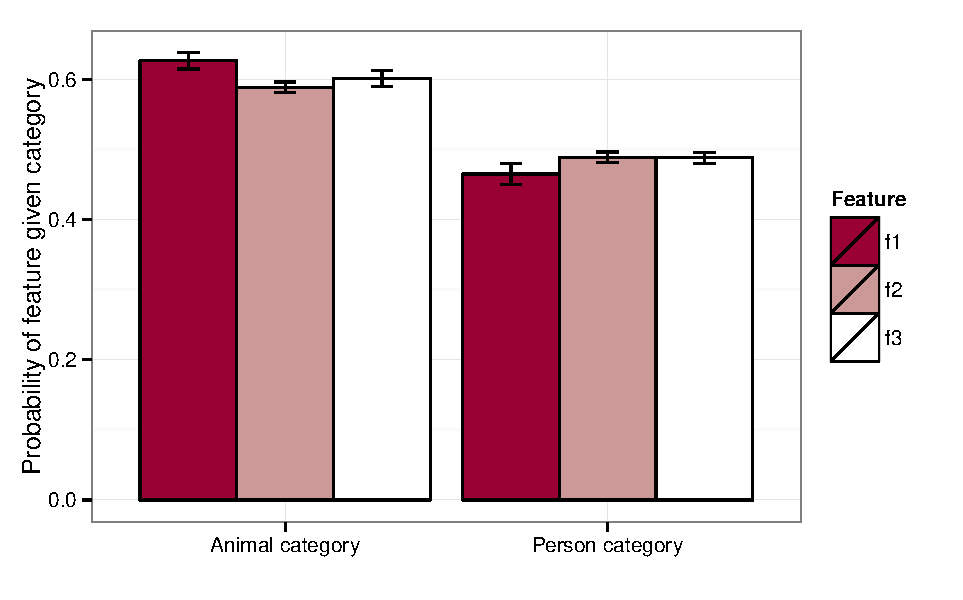
\includegraphics{Plots/prior.pdf}}
\end{center}
\caption{This is a figure.} 
\label{prior}
\end{figure}

\subsubsection{Results} 
We make the simplifying assumption that the eight feature combinations presented in each trial exhaustively describe a member of a particular category. As a result, we normalized each subject's ratings for the eight feature combinations in a trial to sum up to 1. Averaging across subjects' normalized ratings, we obtained the feature priors $P_F(\vec f | c)$ for $c = c_a$ (animal) and $c = c_p$ (person), assuming that $f_i = 1$ is represented by the feature adjective and $f_i = 0$ is represented by the antonym. 

For ease of interpretation, in Table 1 we present the marginal probabilities of each of the three features instead of the joint probabilities. Figure~\ref{prior} shows the average marginal probabilities of features given an animal category versus a person category. We see that by design, features are rated as significantly more likely to be present given the animal category than the person category.

\subsection{Experiment 2: Metaphor Understanding}
\subsubsection{Materials and Methods}
We created $32$ scenarios based on the animal categories and results from Experiment 1. In each scenario, a person (e.g. Bob) is having a conversation with his friend about a person that he recently met. Since we are interested in how relevance to the question under discussion (QUD) affects metaphor interpretation as well as the effectiveness of metaphorical versus literal utterances, we created four conditions for each scenario by crossing vague/specific QUD and literal/metaphorical statements. In vague QUD conditions, Bob's friend asks a vague question about the person Bob recently met: ``What is he like?" In specific QUD conditions, Bob's friend asks a specific question about the person: ``Is he $f1$?" Where $f1$ is the most popular adjective for a given animal category $c_a$ in Experiment 1A. In literal conditions, Bob replies with a literal utterance,, either by saying ``He is $f1$" to the question ``What is he like?" or ``Yes" to the question ``Is he $f1$?". In Metaphorical conditions, Bob replies with a metaphorical statement, e.g. ``He is a $c_a$" where $c_a$ is an animal category. See Table 2 for examples.
 
\subsubsection{Results}
\begin{figure}[ht]
\begin{center}
\scalebox{0.6}{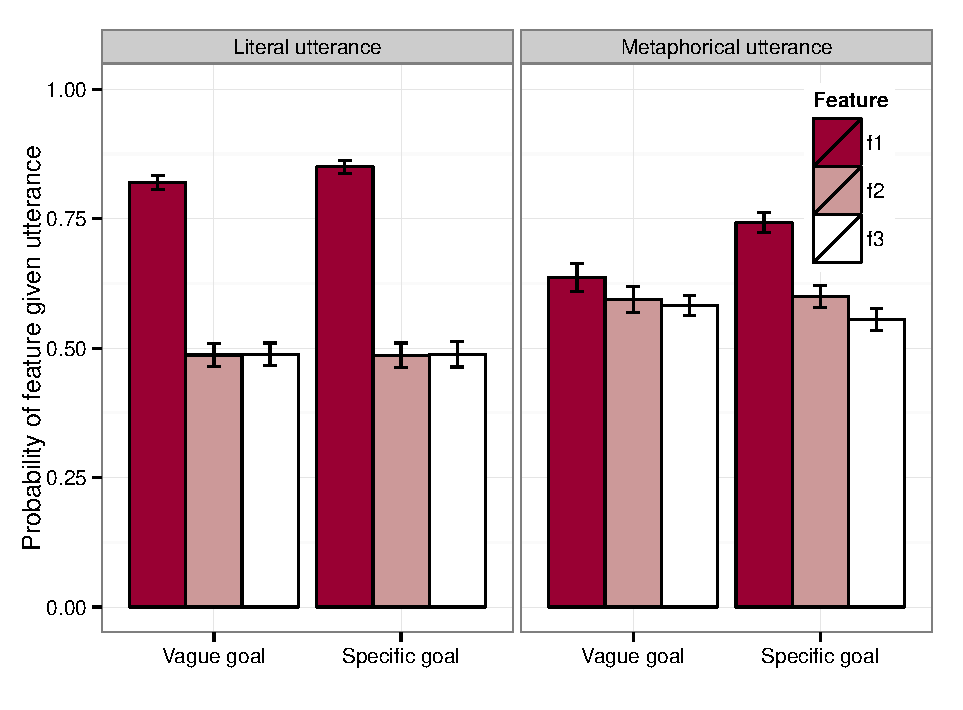
\includegraphics{Plots/human_bar.pdf}}
\end{center}
\caption{This is a figure.} 
\label{human_bar}
\end{figure}

$49$ native English speakers with IP addresses in the United States were recruited on Amazon's Mechanical Turk. Each subject completed $32$ trials in random order. The $32$ trials were randomly and evenly assigned to one of the four conditions, i.e. each subject read $8$ scenarios for each condition. For each trial, subjects used sliders to indicate the probabilities that the person described has features $f1$, $f2$, and $f3$.

For each condition of each scenario, we obtained the average probability ratings for the three features. Figure~\ref{human_bar} shows the average ratings for each feature across animal categories given a vague or specific QUD and a literal or metaphorical utterance. We see that when the speaker gives a literal statement directly affirming the presence of $f1$, subjects rate $f1$ as significantly more likely than when the speaker gives a metaphorical statement. However, subjects rate $f2$ and $f3$ as significantly more likely when the speaker produces a metaphorical utterance. We also see an effect of the QUD on the interpretation of metaphorical utterances. Given a specific question about $f1$, subjects interpret the speaker's metaphorical utterance as being relevant to the question and rates the probability of $f1$ as significantly higher than when the QUD is vague. On the other hand, the probabilities of $f2$ and $f3$ are not significantly different given a vague QUD or a specific QUD about $f1$.

%\section{Model Comparison}
%\begin{figure}[ht]
%\begin{center}
%\scalebox{0.6}{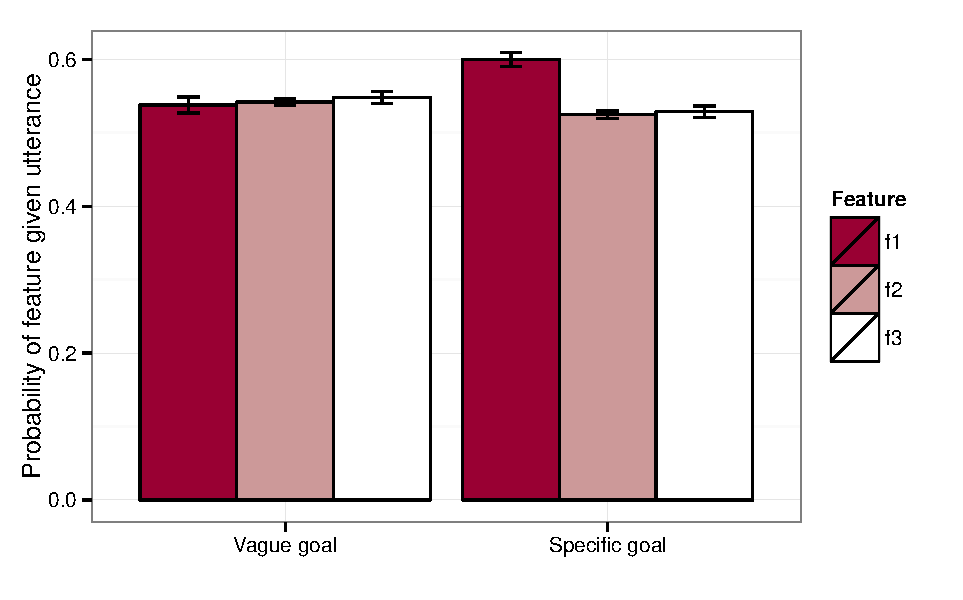
\includegraphics{Plots/model_bar.pdf}}
%\end{center}
%\caption{This is a figure.} 
%\label{model_bar}
%\end{figure}

We used the feature priors obtained in Experiment 1B to compute model interpretations of the $32$ metaphors.
For the category prior $P_C(c)$, we assumed that given the common ground set up by the conversation, it is extremely unlikely for the person described to actually belong to the animal category $(P_C(c_a) = 0.0001)$ and extremely likely for him to belong to the person category $(P_C(c_p) = 0.9999)$. We model the effect of relevance to the question under discussion by assuming that the goal prior $P_G(g | \vec f)$ varies given vague or specific QUDs. When the QUD is vague, we set the distribution as uniform over goals that are consistent with $\vec f$. When the QUD specifically addresses $f_1$, we set the distribution as having a much higher probability for $g_1$ and equal probability for $g_2$ and $g_3$.

Using these prior settings and the model we described, we obtained feature probabilities for each of the $32$ metaphors. Figure~\ref{model_bar} shows the average marginal feature probabilities for the $32$ metaphors given a vague or specific QUD. We see that the model captures the QUD effect, where $f1$ receives a significantly higher probability when the speaker is a priori more likely to be informative about $f1$. (Need to describe results for "literal" statement where it's just the prior.)

To quantitatively evaluate the model's performance on metaphorical utterances, we correlated model predictions with human ratings for each of the features given a metaphorical utterance and a vague or specific QUD. We first focused on the model's performance on $f1$ features, namely the most salient features and ones that can be specifically under discussion. Correlation between human ratings and the model's marginal posterior probabilities for $f1$ across the $32$ metaphors and vague/specific QUD conditions is $0.73$ (add Spearman prophecy formula), suggesting that the model captures a significant amount of the reliable variance in the human data. We then compare this performance with baseline models that only consider feature priors of the source (animal category) or target (person category). A baseline model consisting of only feature priors for the animal categories yields a non-significant correlation ($r=-0.03, p > 0.05$). A baseline model consisting of only feature priors for the person category yields a significant correlation ($r=0.59, p < 0.01$), but one that is significantly worse than the model predictions ($p < 0.001$ with a Cox test). A linear regression model that takes both sets of priors as predictors still yields a significantly worse fit than our model. This suggests that our model adequately combines prior knowledge about the source and target domains to produce metaphor interpretations that closely fit humans'.
\begin{figure}[ht]
\begin{center}
\scalebox{0.6}{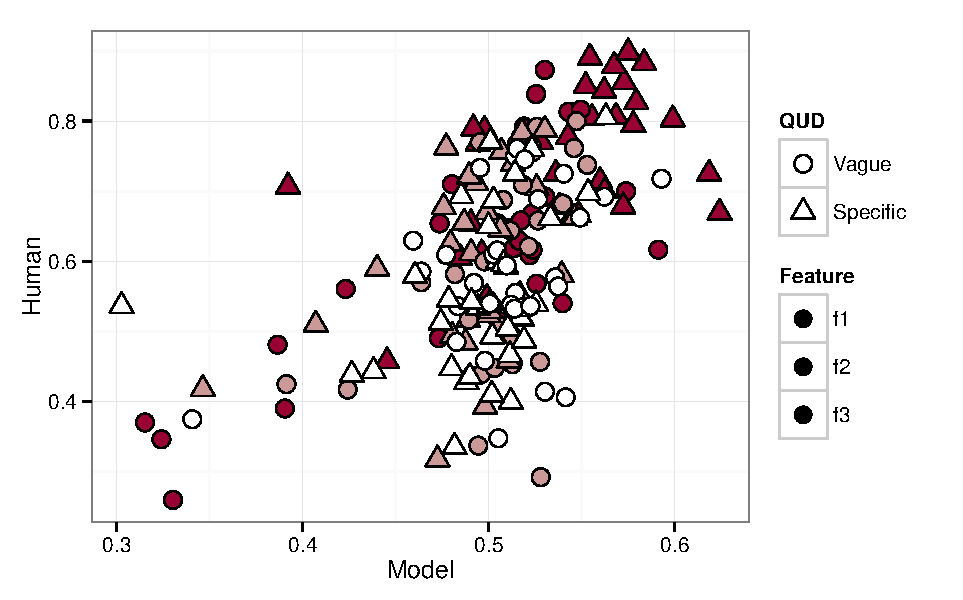
\includegraphics{Plots/scatter_full.pdf}}
\end{center}
\caption{This is a figure.} 
\label{scatter_full}
\end{figure}

We now evaluate the model's performance on all three types of features. Correlation between human ratings and the model's marginal posterior probabilities for $f1$, $f2$, and $f3$ across the $32$ metaphors and vague/specific QUD conditions is $0.56$ (add Spearman prophecy formula). Figure~\ref{scatter_full} shows the model predictions against human ratings for the three features of each metaphor given a vague or specific QUD. While our model still captures a significant amount of reliable variance in the human data, we see that there are certain features, particularly $f2$ and $f3$, for which the model performance is significantly worse. We analyze these metaphors and features in more detail in the following section.






\section{Discussion}
Discuss implication of results on the pragmatics of metaphor; discuss other effects we could explore using the modeling framework; suggest future directions.

In this paper we focus on developing a computational model of pragmatics that explains a range of effects in metaphor understanding, with the goal of advancing our understanding of the computational basis of metaphor and nonliteral language understanding.

Building upon Rational Speech Act models, we present a computational model that predicts rich metaphorical interpretations using basic pragmatic reasoning.

\subsection{Footnotes}


%\subsection{Tables}

%\begin{table}[!ht]
%\begin{center} 
%\caption{Sample table title.} 
%\label{sample-table} 
%\vskip 0.12in
%\begin{tabular}{ll} 
%\hline
%Error type    &  Example \\
%\hline
%Take smaller        &   63 - 44 = 21 \\
%Always borrow~~~~   &   96 - 42 = 34 \\
%0 - N = N           &   70 - 47 = 37 \\
%0 - N = 0           &   70 - 47 = 30 \\
%\hline
%\end{tabular} 
%\end{center} 
%\end{table}


\section{Acknowledgments}

Place acknowledgments (including funding information) in a section at
the end of the paper.



\bibliographystyle{apacite}

\setlength{\bibleftmargin}{.125in}
\setlength{\bibindent}{-\bibleftmargin}

\bibliography{metaphor}


\end{document}
